%----------------------------------------------------------------------------------------
%	PACKAGES AND DOCUMENT CONFIGURATIONS
%----------------------------------------------------------------------------------------

\documentclass[
	a4paper, % Paper size, specify a4paper (A4) or letterpaper (US letter)
	10pt, % Default font size, specify 10pt, 11pt or 12pt
]{report}

\usepackage[utf8]{inputenc}	% UTF-8 encoding
\usepackage[english]{babel} % Document language - required for customizing section titles

\usepackage{biblatex} % Required for bibliography management
\usepackage{hyperref} % For hyperlinks
\hypersetup{
    colorlinks=true,
    linkcolor=black,
}

\usepackage{titlesec} % For custom section numbering format

\usepackage{amsmath, amssymb, amsthm} % Required for some math elements

\usepackage{float} % Allows putting an [H] in \begin{figure} to specify the exact location of the figure
\usepackage{geometry}
\usepackage{textgreek}

\usepackage{graphicx} % Required for the inclusion of images
\usepackage{caption, subcaption} % Required for the inclusion of captions

\usepackage{booktabs} % Required for better horizontal rules in tables

\usepackage{siunitx} % Required for alignment of numbers with units


\geometry{top=3cm} % Adjust the top margin as needed
\geometry{bottom=2.5cm} % Adjust the bottom margin as needed

% Custom section numbering format (without prefix)
\renewcommand{\thesection}{\arabic{section}}

\newcounter{definition}[section] % Define a new counter tied to sections
\renewcommand{\thedefinition}{\thesection.\arabic{definition}} % Customize the counter format

\newenvironment{defn}[1][]{%
    \refstepcounter{definition}% Increment the counter
    \par\medskip\noindent%
    \textbf{Definizione \thedefinition: #1 \\}% Header
}{
    \par\medskip % Insert a break
}


\begin{document}

%----------------------------------------------------------------------------------------
%	REPORT INFORMATION
%----------------------------------------------------------------------------------------

\begin{titlepage}
	\begin{center}

		\vspace{1.5cm} % Adjust vertical space

		
\includegraphics[width=1\textwidth]{figures/unimi.jpg} % University logo

		\vspace{1.5cm} % Adjust vertical space
		
		\Huge Laboratorio di Elettronica \\ Note del corso % Report title
		
		\vspace{1cm} % Adjust vertical space
		
		\Large Lorenzo \textsc{Liuzzo} % Author name(s), add additional authors like: '\& James \textsc{Smith}'
		
		\vspace{2cm} % Adjust vertical space

		\begin{tabular}{l r}
			Bachelor's Degree: & Physics \\ % Degree
			Academic Year: & 2022/2023 \\ % Accademic year
			Course: & Electronics Laboratory \\ % Course
			Professor: & Valentino \textsc{Liberali} \\% Instructor/supervisor
		\end{tabular}

		\vfill % Fill the rest of the page with whitespace
	
	\end{center}
\end{titlepage}


%----------------------------------------------------------------------------------------
%	TABLE OF CONTENTS
%----------------------------------------------------------------------------------------

\tableofcontents % Include a table of contents

\newpage % Begins the essay on a new page instead of on the same page as the table of contents

%----------------------------------------------------------------------------------------
%	SECTION 1
%----------------------------------------------------------------------------------------

\section{Lezione 1}

\begin{defn}[Carica elettrica]
	La carica elettrica \emph{Q} è una proprietà fondamentale della materia che indica il passaggio di corrente elettrica per tempo: $$ \SI{1}{C} = \SI{1}{\ampere\second} $$ \\
	La carica elettrica può essere sia positiva sia negativa, ed è quantizzata, cioè tutte le cariche sono multipli della carica elementare: $$ q = \SI{1.6021e-19}{C} $$  
	Le cariche elettriche sono sempre soggette ad una forza elettrica, detta \emph{di Coulomb}, pari a $$ \vec{F} = \frac{1}{4\pi\varepsilon} \cdot \frac{q_1 q_2}{r^2} \cdot \hat{r} $$
\end{defn}

\begin{defn}[Corrente elettrica]
	La corrente elettrica, o intensità di corrente elettrica, \emph{I}, è data dal movimento di cariche mobili e matematicamente si esprime come la derivata della carica elettrica rispetto al tempo: $$ I = \frac{dQ}{dt} $$
	La corrente si misura in serie con l'amperometro.
\end{defn}

\begin{defn}[Differenza di potenziale]
	La tensione \emph{V} tra due punti è l'integrale di linea del campo elettrico su un percorso qualsiasi che congiunga i due punti: $$ V_{ab} = \int_a^b \vec{E} \cdot \vec{dl} $$
	La tensione si misura in parallelo con il voltmetro.
\end{defn}

\begin{defn}[Potenza]
	La potenza \emph{P} è il prodotto tra la tensione e la corrente: $$ P = V I $$
	La potenza si misura in watt. Ha segno positivo se il bipolo aumenta l'energia immagazzinata, negativo se la diminuisce.
\end{defn}

\begin{defn}[Energia elettrica]
	L'energia elettrica viene distribuita attraverso la rete di distribuzione con un sistema trifase a quattro conduttori: tre hanno tensioni sinusoidali sfasate tra loro di $\frac{2\pi}{3}$, il quarto, detto neutro, è collegato a terra e costituisce il potenziale zero di riferimento. Il valore medio della tensione di rete è zero, mentre il valore efficace (root-mean-square rms) è 230 V. 
	Le apparecchiature elettriche devono rispettare determinate specifiche di sicurezza: 
	\begin{itemize}
		\item classe I: messa a terra di protezione \\
		un circuito elettrico monofase ha tutte le parti in tensione isolate per il livello di tensione nominale, mentre l'involucro metallico dell'apparecchiatura è collegato a terra. Inoltre, sono posizionati due interruttori differenziali (o salvavita) che rilevino lo squilibrio tra la corrente di fase e la corrente di guasto. Un interruttore differenziale deve aprire il circuito quando la differenza tra le correnti è maggiore o uguale a 30 mA, cioè la soglia di pericolosità della corrente per il corpo umano. 
		\item classe II: doppio isolamento \\
		Gli apparecchi a doppio isolamento non richiedono la messa a terra e sono costruiti in modo che un singolo guasto non possa causare il contatto con tensioni pericolose.
		\item classe III: bassissima tensione di sicurezza \\
		Una tensione non superiore a 25 V in alternata o 50 V in continua non rappresenta un pericolo per il corpo umano. Si consiglia di non superare il $\pm$ 12 per i circuiti che vedremo in laboratorio. 
	\end{itemize}
\end{defn}

\begin{defn}[Bipoli elettrici]
	I circuiti elettrici sono formati da elementi circuitali interconnessi tra di loro. I più semplici elementi circuitali sono dispositivi a due terminali, o bipoli. \\
	Al bipolo è applicata la differenza di potenziale \emph{V} e attraverso di esso fluisce la corrente elettrica \emph{I}. I due terminali vengono contrassegnati con i simboli \emph{+} ed \emph{-}. 
	La tensione si misura dal polo negativo a quello positivo. La corrente si considera positiva quando entra nel bipolo \emph{+}. 
\end{defn}

\begin{defn}[Nodo]
	Un nodo è un punto di un circuito elettrico in cui si incontrano due o più bipoli.
\end{defn}

\begin{defn}[Maglia]
	Una maglia è un percorso chiuso attraverso due o più bipoli di un circuito.
\end{defn}

\begin{defn}[Resistore e legge di Ohm]
	Il più semplice bipolo lineare è il resistore, caratterizzato da proporzionalità diretta tra tensione e corrente (\emph{Legge di Ohm}): 
	$$ V = R I $$ dove R è la resistenza che si misura in Ohm: $$ 1 \Omega = 1 V/A = 1 kg m^2 / (A^2 s^3) $$
\end{defn}

\begin{defn}[Generatori]
	Un generatore è un bipolo attraverso 
	Un generatore di tensione presenta una tensione fissata fra i suoi terminali. Il più semplice generatore di tensione constante nel tempo è una pila o batteria. 
\end{defn}

\begin{defn}[Multimetro]
	Un multimetro è uno strumento di misurazione in grado di misurare tensione, corrente e resistenza. I multimetri possono essere analogici e digitali, palmari o da banco. \\
	La corrente (sia in alternata sia in continua) si misura in serie, quindi bisogna aprire il circuito ed inserire l'amperometro in serie. \\
	La tensione (sia in alternata sia in continua) si misura in parallelo, quindi bisogna mettere in parallelo il voltmetro. Misurare la tensione è più comodo rispetto alla misura di corrente. \\
\end{defn}

\begin{defn}[Alimentatore]
	Un alimentatore funziona in modo simile ad un generatore ideale e forniscono una differenza di potenziale di circa 30 V. Se vogliamo una corrente o positiva o negativa, si effettua manualmente un collegamento a terra tra il terminale e l'alimentatore. 
\end{defn}

\begin{defn}[Partitore di tensione]
	Un partitore di tensione è costituito da due o più componenti passivi collegati in serie. Se ai capi della serie viene applicata una tensione, essa si ripartirà ai capi dei componenti in base al loro valore. 
\end{defn}


\begin{defn}[Cortocircuito]
	Il cortocircuito è un collegamento tra due nodi effettuato con un generatore di tensione nulla. In un cortocircuito la tensione ai capi del generatore è nulla, quindi la corrente può assumere qualsiasi valore.
\end{defn}

\begin{defn}[Circuito aperto]
	Un generatore di corrente spento è percorso da una corrente nulla e tensione qualsiasi.
	Il circuito aperto è un collegamento tra due nodi effettuato con un generatore di corrente nulla.
\end{defn}

\begin{defn}[Leggi di Kirchhoff]
	La somma algebrica delle correnti in un nodo di un circuito è zero: $$ \sum_{i} I_i = 0 $$
	La somma algebrica delle tensioni in una maglia di un circuito è zero: $$ \sum_{j} V_j = 0 $$
\end{defn}

\begin{defn}[Partitore di tensione]
	Un partitore di tensione è costituito da due o più componenti passivi collegati in serie.
	Se ai capi della serie viene applicata una tensione, essa si ripartirà ai capi dei componenti in base al loro valore.
	\begin{figure}[H]
		\centering
		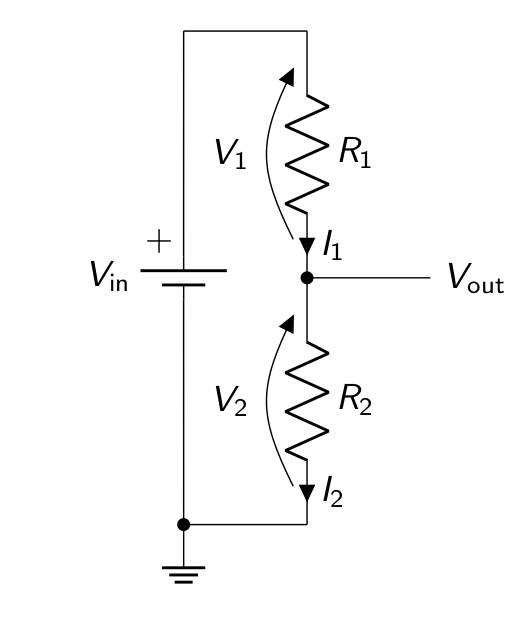
\includegraphics[width=0.5\linewidth]{figures/partitore_tensione.png}
		\caption{Partitore di tensione}
		\label{fig:partitore_tensione}
	\end{figure}
\end{defn}


\section{Grandezze elettriche variabili nel tempo, consensatore e induttore, circuiti RC del primo ordine}

\begin{defn}[Segnale]
    Una grandezza elettrica che varia nel tempo secondo una legge determinata costituisce un segnale. 
    I segnali possono essere di tensione oppure di corrente. \\
    Un segnale è analogico quando il suo contenuto di informazione varia con
    continuità, potendo assumere un'infinità di valori possibili (entro un certo intervallo).
    Un segnale è digitale quando il suo contenuto di informazione varia in modo discreto, 
    potendo assumere soltanto un numero finito di valori possibili. \\
    Un segnale è periodico quando si ripete identicamente dopo un intervallo di tempo detto periodo.
\end{defn}

\begin{defn}[Valore medio e valore efficace]
    Il valore medio di un segnale periodico è il valore medio di una sua singola oscillazione: 
    $$V_{med} = \frac{1}{T} \int_{0}^{T} V(t) dt$$
    Il valore efficace di un segnale periodico è il valore della tensione continua che, applicata ad un resistore, 
    produce la stessa potenza dissipata dal resistore stesso quando è attraversato dal segnale periodico: 
    $$V_{eff} = \sqrt{\frac{1}{T} \int_{0}^{T} V^2(t) dt}$$
\end{defn}

\begin{defn}[Energia interna]
    Elementi circuitali il cui comportamento non dipende solo dal valore instantaneo delle grandezze elettriche, 
    ma anche dai valori assunti in precedenza, mantengono al loro interno un'informazione legata al loro funzionamento passato.
    L'informazione è fisicamente immagazzinata sotto forma di energia variabile nel tempo $w(t)$. 
    L'energia assorbita da un bipolo all'istante t è: $$w(t) = \int_{-\infty}^{t} p(\tau) d\tau$$
\end{defn}

\begin{defn}[Condensatore]
    Il condensatore è costituito da due superfici metalliche parallele separate da un isolante. 
    La carica immagazzinata è proporzionale alla tensione applicata: $$q(t) = C v(t)$$
    La costante C è la capacità del condensatore, che si misura in farad (F): $$\SI{1}{\farad} = \SI{1}{\coulomb\per\volt}$$
    Per un condensatore a facce piane e parallele di area $S$ poste ad una distanza $d$ l'una dall'altra, 
    con un dielettrico di costante dielettrica relativa $\epsilon$, la capacità è: $$C = \frac{\epsilon S}{d}$$
	\begin{figure}[H]
		\centering
		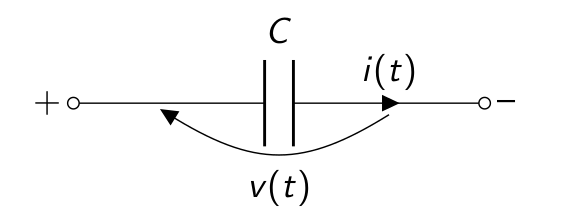
\includegraphics[width=0.5\linewidth]{figures/condensatore.png}
		\caption{Condensatore}
		\label{fig:condensatore}
	\end{figure}
    \noindent Nel condensatore la corrente è proporzionale alla derivata della tensione: $$i(t) = C \frac{dv(t)}{dt}$$
    mentre la tensione è proporzionale all'integrale della corrente: $$v(t) = \frac{1}{C} \int_{0}^{t} i(\tau) d\tau + v(0)$$
    L'energia immagazzinata nel condensatore è: $$w(t) = \frac{1}{2} C v^2(t)$$
    mentre la potenza instantanea è: $$p(t) = \frac{dw(t)}{dt} = C v(t) \frac{dv(t)}{dt}$$
\end{defn}

\begin{defn}[Induttore e legge di Faraday-Henry]
    L'induttore è costituito da un avvolgimento di filo conduttore, detto solenoide.
    All'interno dell'avvolgimento si ha un flusso magnetico $\Phi$ proporzionale alla corrente nel filo: $$\Phi(t) = L i(t)$$
    La constante $L$ è l'induttanza dell'induttore, che si misura in henry (H): $$\SI{1}{\henry} = \SI{1}{\volt\second\per\ampere}$$
	\begin{figure}[H]
		\centering
		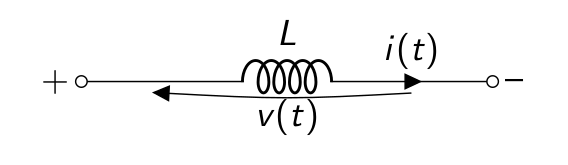
\includegraphics[width=0.5\linewidth]{figures/induttore.png}
		\caption{Induttore}
		\label{fig:induttore}
	\end{figure}
    \noindent Una variazione nel tempo del flusso magnetico produce una differenza di potenziale ai capi dell'induttore (legge di Faraday-Henry):
    $$v(t) = L \frac{di(t)}{dt}$$
    La tensione è dunque proporzionale alla derivata della corrente, mentre la corrente è proporzionale all'integrale della tensione:
    $$i(t) = \frac{1}{L} \int_{0}^{t} v(\tau) d\tau + i(0)$$
    L'energia immagazzinata nell'induttore è: $$w(t) = \frac{1}{2} L i^2(t)$$
    quindi la potenza instantanea è: $$p(t) = L i(t) \frac{di(t)}{dt}$$
\end{defn}


\section{Trasformata di Fourier, risposta in frequenza e diagrammi di Bode}

% \begin{defn}[]
% Ogni segnale x(t) periodico con periodo T = f10 può essere espresso come serie di
% Fourier:

\section{Amplificatore operazionale}

\begin{defn}[Generatori dipendenti]
    Un generatore dipendente è un elemento che genera una grandezza elettrica (tensione o corrente) il cui valore è funzione di
    un'altra grandezza elettrica (tensione o corrente) presente nel circuito.
    I generatori dipendenti sono “doppi bipoli”, cioè hanno una coppia di terminali di ingresso per la variabile di controllo e 
    una coppia di terminali di uscita per la grandezza generata. 
    Convenzionalmente, nelle figure i terminali di ingresso sono a sinistra e i terminali di uscita sono a destra.
\end{defn}

\begin{defn}[Generatore di tensione controllato in tensione]
	All'ingresso non assorbe corrente (si comporta come un circuito aperto).\\
	Il parametro $E$ è il guadagno di tensione (adimensionale): $E = V_o / V_i$
	\begin{figure}[H]
		\centering
		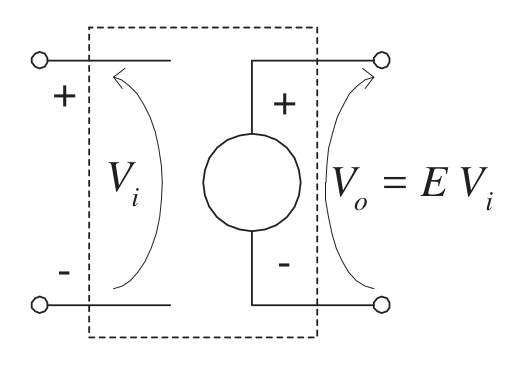
\includegraphics[width=0.5\linewidth]{figures/VCVS.png}
		\caption{VCVS}
		\label{fig:VCVS}
	\end{figure}
\end{defn}

\begin{defn}[Generatore di corrente controllato in corrente]
	All'ingresso non c'è caduta di tensione (si comporta come un cortocircuito). \\
	Il parametro $F$ è il guadagno di corrente (adimensionale): $F = I_o / I_i$
	\begin{figure}[H]
		\centering
		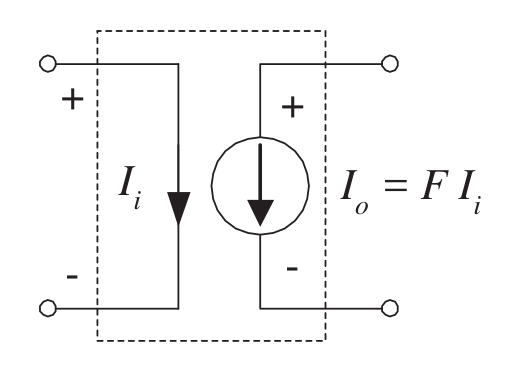
\includegraphics[width=0.5\linewidth]{figures/CCCS.png}
		\caption{CCCS}
		\label{fig:CCCS}
	\end{figure}
\end{defn}

\begin{defn}[Generatore di corrente controllato in tensione]
	All'ingresso non assorbe corrente (circuito aperto). \\
	Il parametro $G$ è la transconduttanza, o conduttanza di trasferimento tra ingresso e uscita, che dimensionalmente è una conduttanza e si misura in Siemens:
	$G = I_o / V_i$
	\begin{figure}[H]
		\centering
		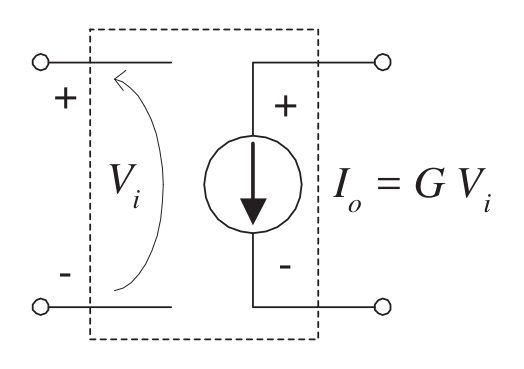
\includegraphics[width=0.5\linewidth]{figures/VCCS.png}
		\caption{VCCS}
		\label{fig:VCCS}
	\end{figure}
\end{defn}

\begin{defn}[Generatore di tensione controllato in corrente]
	All'ingresso non c'è caduta di tensione (cortocircuito). \\
	Il parametro $H$ è la transresistenza o resistenza di trasferimento tra ingresso e uscita, che dimensionalmente è una resistenza e si misura in Ohm:
	$H = V_o / I_i$
	\begin{figure}[H]
		\centering
		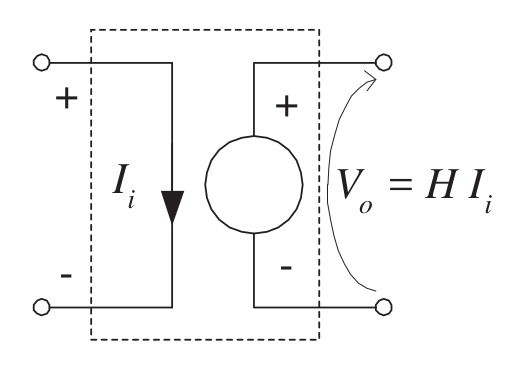
\includegraphics[width=0.5\linewidth]{figures/CCVS.png}
		\caption{CCVS}
		\label{fig:CCVS}
	\end{figure}
\end{defn}


\section{Circuiti con amplificatori operazionali}


\section{Lezione 6}


\section{Lezione 7}


\section{Lezione 8}


\section{Tecnologia CMOS}




\end{document}